\documentclass{beamer}
\usepackage[utf8]{inputenc}
\usepackage{booktabs}
\usepackage{tabulary}
\usetheme{simple}
\usecolortheme{whiteonblack}
\title{Semantic MediaWiki}
\subtitle{Good for authoring Linked Data?}
\author{Konrad Höffner}

\begin{document}
\begin{frame}
\titlepage
\end{frame}

\begin{frame}{Situation: We generate and maintain Linked Data}
\centering
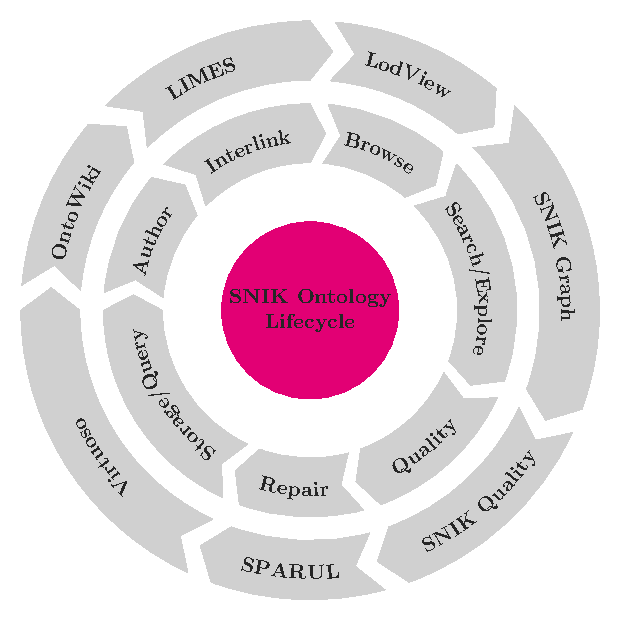
\includegraphics[width=0.8\textwidth]{cycle.pdf}
\end{frame}

\begin{frame}{Our data constantly changes}
\centering
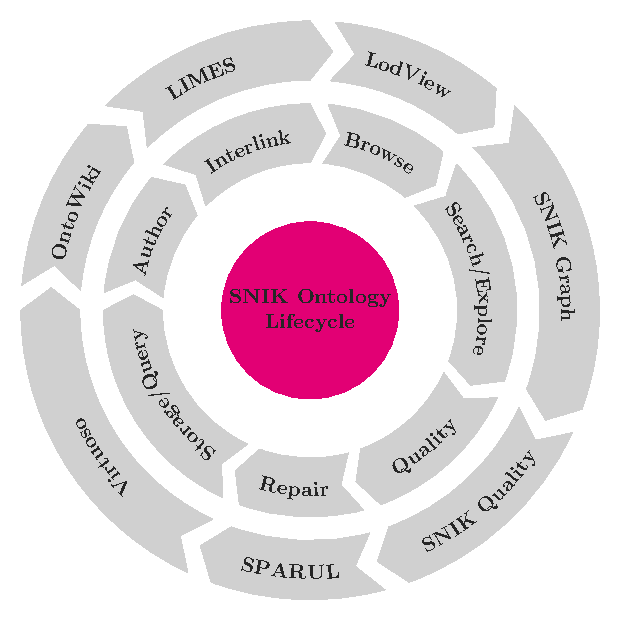
\includegraphics[width=0.8\textwidth]{cycle.pdf}
\end{frame}

\begin{frame}{Problem: Authoring isn't easy}
\centering
\includegraphics[width=0.8\textwidth]{cycle-red.pdf}
\end{frame}

\begin{frame}{Problem: Authoring isn't easy}
\centering
\begin{tabulary}{\textwidth}{lLL}
\toprule
Tool		&Pros						&Cons\\
\midrule
Text Editor	&speed, version control, close to the metal	&requires Turtle \& Git skills\\
SPARUL		&many changes at once 				&requires SPARUL syntax\\
Prot\'eg\`e	&\\
\bottomrule
\end{tabulary}
\end{frame}

\begin{frame}{Problem: Authoring isn't easy}
\centering
\begin{tabulary}{\textwidth}{lLL}
\toprule
Tool		&Pros						&Cons\\
\midrule
Text Editor	&speed, version control, close to the metal	&requires Turtle \& Git skills\\
SPARUL		&many changes at once 				&requires SPARUL syntax\\
Prot\'eg\`e	&\\
\bottomrule
\end{tabulary}
\end{frame}

\begin{frame}{Problem}
\begin{itemize}
\item we have a bunch of Linked Data
\item technical users can use SPARUL queries or edit TURTLE syntax
\item 
\item 
\item 
\item 
\end{itemize}
\end{frame}
\end{document}

\begin{frame}{Bla}
\begin{itemize}
\item blabla
\item 
\item 
\item 
\item 
\end{itemize}
\end{frame}
\end{document}

\begin{frame}{Bla}
\begin{itemize}
\item blabla
\item 
\item 
\item 
\item 
\end{itemize}
\end{frame}
\end{document}

\begin{frame}{Bla}
\begin{itemize}
\item blabla
\item 
\item 
\item 
\item 
\end{itemize}
\end{frame}
\end{document}

\begin{frame}{Bla}
\begin{itemize}
\item blabla
\item 
\item 
\item 
\item 
\end{itemize}
\end{frame}
\end{document}
